\documentclass{standalone}
\usepackage{tikz}

\begin{document}

\begin{tikzpicture}
    % First linear realization
    \foreach \x in {0,1,2,3,4,5,6} {
        \node[draw, circle, inner sep=1pt, fill=black] at (\x, 0) {};
    }
    \foreach \x in {7,8,9,10,11,12,13,14,15,16,17,18,19,20} {
        \node[draw, circle, inner sep=1pt, fill=black] at (\x-7, 1) {};
    }
    \foreach \x in {21,22,23,24} {
        \node[draw, circle, inner sep=1pt, fill=black] at (\x-21, 2) {};
    }
    \draw (0,0) -- (6,0) -- (6,1) -- (0,1) -- (0,0);
    \draw (1,0) -- (1,1);
    \draw (2,0) -- (2,1);
    \draw (3,0) -- (3,1);
    \draw (4,0) -- (4,1);
    \draw (5,0) -- (5,1);
    \draw (6,0) -- (6,1);
    \draw (0,1) -- (0,2) -- (3,2) -- (3,1);
    \draw (4,1) -- (4,2) -- (6,2);

    \foreach \x/\y in {0/0, 1/1, 2/2, 3/3, 4/4, 5/5, 6/6, 7/7, 8/8, 9/9, 10/10, 11/11, 12/12, 13/13, 14/14, 15/15, 16/16, 17/17, 18/18, 19/19, 20/20, 21/21, 22/22, 23/23, 24/24} {
        \node[anchor=north] at (\y,0) {\x};
    }
    \node[anchor=north] at (0,1) {7};
    \node[anchor=north] at (1,1) {8};
    \node[anchor=north] at (2,1) {9};
    \node[anchor=north] at (3,1) {10};
    \node[anchor=north] at (4,1) {11};
    \node[anchor=north] at (5,1) {12};
    \node[anchor=north] at (6,1) {13};
    \node[anchor=north] at (0,2) {21};
    \node[anchor=north] at (1,2) {22};
    \node[anchor=north] at (2,2) {23};
    \node[anchor=north] at (3,2) {24};

    % Second linear realization
    \begin{scope}[xshift=10cm]
        \foreach \x in {0,1,2,3,4,5,6,7} {
            \node[draw, circle, inner sep=1pt, fill=black] at (\x, 0) {};
        }
        \foreach \x in {8,9,10,11,12,13,14,15,16,17} {
            \node[draw, circle, inner sep=1pt, fill=black] at (\x-8, 1) {};
        }
        \foreach \x in {18,19,20,21,22,23,24,25,26,27} {
            \node[draw, circle, inner sep=1pt, fill=black] at (\x-18, 2) {};
        }
        \draw (0,0) -- (7,0) -- (7,1) -- (0,1) -- (0,0);
        \draw (1,0) -- (1,1);
        \draw (2,0) -- (2,1);
        \draw (3,0) -- (3,1);
        \draw (4,0) -- (4,1);
        \draw (5,0) -- (5,1);
        \draw (6,0) -- (6,1);
        \draw (7,0) -- (7,1);
        \draw (0,1) -- (0,2) -- (3,2) -- (3,1);
        \draw (4,1) -- (4,2) -- (6,2);
        \draw (6,1) -- (6,2);
        \draw (7,1) -- (7,2);
        
        \foreach \x/\y in {0/0, 1/1, 2/2, 3/3, 4/4, 5/5, 6/6, 7/7, 8/8, 9/9, 10/10, 11/11, 12/12, 13/13, 14/14, 15/15, 16/16, 17/17, 18/18, 19/19, 20/20, 21/21, 22/22, 23/23, 24/24, 25/25, 26/26, 27/27} {
            \node[anchor=north] at (\y,0) {\x};
        }
        \node[anchor=north] at (0,1) {7};
        \node[anchor=north] at (1,1) {8};
        \node[anchor=north] at (2,1) {9};
        \node[anchor=north] at (3,1) {10};
        \node[anchor=north] at (4,1) {11};
        \node[anchor=north] at (5,1) {12};
        \node[anchor=north] at (6,1) {13};
        \node[anchor=north] at (7,1) {14};
        \node[anchor=north] at (0,2) {22};
        \node[anchor=north] at (1,2) {23};
        \node[anchor=north] at (2,2) {24};
        \node[anchor=north] at (3,2) {25};
        \node[anchor=north] at (4,2) {26};
        \node[anchor=north] at (5,2) {27};
    \end{scope}
\end{tikzpicture}

\end{document}